% !TEX root = ../main.tex


\section{Run To Completion}

\emph{Describe Run to completion semantic leading to our Event-B implementation in Basis.}
The run to completetion sematics is implemented via basis that is extend by the model.
\begin{figure}[!h]
	\vspace{-.4cm}
	\centering
	\includegraphics[width=0.99\textwidth]{figures/basis.png}
	\caption{Abstract representation of run to completion basis}
	\label{fig:basis}
	\vspace{-.4cm}
\end{figure}

